
%	Documentação do Trabalho Prático 1 de AEDSIII
%	@Sandro Miccoli
%
%	* Você pode identificar erros de grafia através do seguinte comando linux:
%		aspell --encoding="utf-8" -c -t=tex --lang="pt_BR" tp1.tex
%

\documentclass[12pt]{article}
\usepackage{sbc-template}
\usepackage{float}
\usepackage{graphicx}
\usepackage{latexsym}
\usepackage{changepage}   % for the adjustwidth environment
\usepackage{subfigure}
\usepackage{times,amsmath,epsfig}
\usepackage{graphicx,url}
 \makeatletter
 \newif\if@restonecol
 \makeatother
 \let\algorithm\relax
 \let\endalgorithm\relax
\graphicspath{{./data/}}
\usepackage[lined,algonl,ruled]{algorithm2e}
\usepackage{multirow}
\usepackage[brazil]{babel}
\usepackage[utf8]{inputenc}
\usepackage{listings}

\usepackage{alltt}
\renewcommand{\ttdefault}{txtt}

\sloppy

\title{Programação Modular \\ Trabalho Final \\ Visualização Interativa de Agentes Inteligentes}

\author{Daniel Diniz - 2008046090 - danieldiniz@dcc.ufmg.br\\
		Diogo Santana - 2011054308 - diogo.marques@dcc.ufmg.br\\
		Frederico Figueiredo - 2010054371 - fredfig@dcc.ufmg.br\\
		Sandro Miccoli - 2009052409 - smiccoli@dcc.ufmg.br}

\address{Departamento de Ciência da Computação -- Universidade Federal de Minas Gerais (UFMG)\\
\\
\today}


\begin{document}

\maketitle


\begin{resumo}

Esse relatório descreve como foi implementado a Visualização Interativa de Agentes Inteligentes, proposto como tema para o Trabalho Final. A Seção \ref{introducao} introduz o problema proposto e dá uma visão geral da solução implementada. Cada seção irá descrever detalhes do sistema desenvolvido, abrangendo desde o planejamento (Seção \ref{planejamento}), as decisões de implementação (Seção \ref{implementacao}) e os testes realizados (Seção \ref{testes}). Finalmente concluímos (Seção \ref{conclusao}) a documentação com reflexões sobre o aprendizado durante a execução do trabalho.

\end{resumo}

\section{Introdução}
\label{introducao}

Durante as aulas da disciplina vimos muitos exemplos de como implementar formas geométricas dinâmicas, então decidimos aplicar isso no nosso trabalho final. O objetivo do trabalho é unir os conceitos que aprendemos sobre programação modular e padrões de projeto e aplicá-los num contexto que seja esteticamente agradável. Isso será feito utilizando apenas formas geométricas e linhas com o intuito de gerar padrões visuais interessantes.
O modo como chegaremos nesse resultado será utilizando algoritmos de movimentação de inteligência artificial, usando conceitos como bug algorithm, campos de potencial e desvio de obstáculos (steering).
O planejamento inicial consiste em construir agentes inteligentes que se atraem e repelem. Cada grupo de agentes terá uma atração a certo grupo e repulsão a outros. Por causa dessa característica de atração e repulsão, no momento em que vários agentes são atraídos por um único agente, é esperado que eles entrem em equilíbrio e formem padrões geométricos regulares.
Já é possível perceber várias possibilidades de utilização de padrões de projeto:  Flyweight, caso instanciarmos muitos elementos gráficos; Factory Method, para a geração de diferentes tipos de agentes; State, para definir e controlar dinamicamente o estado de cada agente.

Modelagem inicial do problema.
Construção de agentes básicos.
Implementação do bug algorithm com campos de potencial.
Implementar comportamentos aleatórios para os agentes.
Implementação de uma interface gráfica
Escrever documentação do projeto

Possível utilizar a biblioteca controlP5 do Processing, que permite alterar valores do código em tempo de execução.


O problema proposto neste trabalho foi a especificação e implementação de uma visualização jogo de cartas a ser escolhido pela dupla. O jogo escolhido por nós foi o Pôquer Chinês (Big Two). O objetivo principal do jogo é vencer ao acabar com todas as cartas da mão recebida pelo jogador. A proposta do trabalho prático é proporcionar uma interface simples por linha de comando que seja jogável. O programa implementado será detalhado superficialmente aqui, porém a (Seção \ref{implementacao}) irá explicar em profundo os detalhes de implementação.

\section{Planejamento}
\label{planejamento}

O planejamento que antecedeu à implementação ocorreu da seguinte forma: estudamos as regras do jogo existentes na internet, como são muitas variantes, tivemos que escolher uma e implementar ela. Após isso, definimos os módulos principais que o jogo deveria ter, suas classes e métodos. Com isso, geramos um diagrama UML para melhor compreensão do que iríamos desenvolver. Além disso criamos um repositório git online para que pudéssemos trabalhar em paralelo no mesmo código e caminhar rápido com o trabalho.

\section{Regras}
\label{regras}

O Pôquer Chinês \cite{bigtwo} é um jogo de cartas cujo objetivo é ser o primeiro a desfazer de todas as suas cartas. É por vezes chamada de pôquer chinês devido à sua origem chinesa e uso de mãos de pôquer, embora seja um jogo de natureza completamente diferente.
Ele é jogado tanto casualmente como por dinheiro. É geralmente jogado com dois a quatro jogadores, com o baralho inteiro sendo distribuído para todos os jogadores, ou 13 cartas para cada jogador.
Após as cartas terem sido distribuídas, no geral, o jogador com a menor carta, o 3 de ouros, joga primeiro, com o jogo prosseguindo em uma direção horária. Cartas podem ser colocadas na mesa como únicas, duplas, trios ou em grupo de cinco, utilizando as regras do pôquer, inclusive na primeira jogada feita por quem tem o 3 de ouros.
Depois do início do jogo dado pela jogada do primeiro jogador, o jogador a seguir precisa colocar um mesmo número de cartas que sejam maiores do que aqueles colocados pelo jogador anterior. Caso um jogador não possa ou não queira colocar uma carta ou combinação, ele passa seu turno. Caso todos os oponentes decidam passar, então o jogador remanescente possui o direito de colocar qualquer combinação permitida. O naipe das cartas é utilizado como critério de desempate, sendo a ordem do menor para o maior: ouros, paus, copas e espadas.

\subsection{Tipos de combinações de jogo}
\vspace{0.2 true cm}

Essa subseção irá listar todas as possíveis combinações de jogo.

\begin{description}

\item[Uma carta] \hfill \\
 Qualquer carta do baralho, ordenadas pelo valor da carta (sendo 3 o menor e 2 o maior), com o naipe sendo o critério de desempate. Por exemplo, o 2 de espadas é maior do que qualquer outra carta do jogo, o A de espadas é maior do que o A de ouros, esta sendo maior do que um K de espadas.

\vspace{0.4 true cm}

\item[Par] \hfill \\
 Quaisquer duas cartas iguais, com o maior naipe das duplas sendo utilizado como critério de desempate. Um par de K de espadas e K de ouros é melhor que um par de K de copas e K de paus.

\vspace{0.4 true cm}

\item[Trinca] \hfill \\
 Três cartas de mesmo valor, o desempate é feito através do maior valor.

\vspace{0.4 true cm}

\item[Cinco cartas] \hfill \\
 Existem cinco mãos válidas, ordenadas a seguir do menor para o maior:
 \vspace{0.02 true cm}
\begin{adjustwidth}{1.2cm}{}
\item[\textbf{Sequência}] \hfill \\
		Cinco cartas em sequência, não do mesmo naipe. Caso empate ganha aquele com a maior sequência: 10-J-Q-K-A \textgreater  … \textgreater  2-3-4-5-6 \textgreater  A-2-3-4-5, ou seja, o rank da maior carta da sequência determina qual é a maior, o A e o 2 nas sequências baixas não influenciam no valor da sequência;
\vspace{0.4 true cm}
\item[\textbf{Flush}] \hfill \\
		Cinco cartas do mesmo naipe, não em sequência. O desempate é determinado primeiro pela carta de maior valor, e então pelo naipe mais alto;
\vspace{0.4 true cm}
\item[\textbf{Full House}] \hfill \\
		Uma trinca e um par, a trinca mais alta é utilizada como critério de desempate;
\vspace{0.4 true cm}
\item[\textbf{Quadra + 1}] \hfill \\
		Quatro cartas do mesmo valor mais uma carta qualquer. Observe que, ao contrário do pôquer, uma quadra não pode ser utilizada por sí só. O desempate é determinado pelo valor de uma das cartas da quadra.
\vspace{0.4 true cm}
\item[\textbf{Sequência de mesmo naipe}] \hfill \\
		Uma sequência e um flush ao mesmo tempo. O desempate é determinado primeiro pela maior carta, e então pelo maior naipe.
\vspace{0.4 true cm}
\item[\textbf{Sequência real}] \hfill \\
		O mesmo que a sequência de mesmo naipe, mas limitado a 10, J, Q, K e A. Esta é a maior combinação possível. Apenas uma sequência real com um naipe maior pode vencer outra sequência real. A sequência real de espadas é a combinação de cartas mais poderosa do jogo.
\end{adjustwidth}

\end{description}

\section{Implementação}
\label{implementacao}

Para a implementação dessa simulação utilizamos duas biblioteca de classes Java, \textbf{Processing} e \textbf{ControlP5}. O conjunto de
funções presentes nas classes do Processing facilitam o desenvolvimento de aplicativos orientados a arte visual e contextos gráficos em geral,
enquanto as presentes em ControlP5 nada mais que auxiliam a implementação de controladores para elementos integrados às bibliotecas do Processing. 

Foram utilizados neste sistema os padrões de projeto \textit{Singleton, Decorator e Observer}, de modo a garantir uma melhor modularização do código.
O primeiro foi utilizado para assegurar uma única instância da classe responsável pela apresentação gráfica do sistema, bem como facilitar sua
recuperação e referenciamento por outras classes do aplicativo. O mesmo padrão foi utilizado para tratar a instanciação da classe ControlP5Panel,
garantindo que quaisquer alterações feitas no painel ou qualquer informação que seja buscada por outras classes partirá de uma única instância
unificada deste, tornando-o escalável, dinamicamente modificável, estável e persistente. 

Neste painel pode se constatar, também, a aplicação do padrão \textit{Observer}. Durante a instanciação do Singleton, é criado um elemento nominado
\textit{CallbackListener}, que escuta por interações do tipo \textit{ACTION\_PRESSED} nos elementos do painel de controle, capturados apenas na instância gráfica
principal do aplicativo. Essas interações são então convertidas na forma de eventos e enviados de volta para tratamento na classe do \textbf{P5ControlPanel}.
Tudo isso a fim de garantir que as devidas funções permaneçam encapsuladas de acordo com os princípios de modularidade.

O padrão Decorator por sua vez foi implementado objetivando limitar o número de alterações necessárias na forma básica - \textit{circle} - e
permitir que novos incrementos de formas e comportamentos sejam feitos respeitando os conceitos fundamentais de Orientação a Objetos, ou seja,
grande escalabilidade com o mínimo de alteração nas classes mais abstratas e estáveis. 

A interface (Shape) representa uma forma geométrica que pode ser 'decorada' com uma infinidade de elementos diferentes. Nesse projeto
implementamos apenas diferentes tipos de círculos, tratados para todas as finalidades como comportamentos que decoram os círculos. A simulação conta com
diversas instâncias da forma \textit{circle}, que são independentemente decoradas com o devido comportamento de acordo com a interação realizada pelo usuário
através do painel de controle. Tais forças extendem a classe DecoratorShape, adicionando funcionalidade e efetivamente implementando à interface Shape.

Tudo isso é então colocado em execução sincrôna na classe Main, que sobrescreve funcionalidades implementadas na biblioteca processing para criar uma thread
que monta a simulação com as configurações iniciais e mantém todos os elementos em constante atualização e movimento.

Segue o diagrama de classes simplificado do sistema:

\begin{figure}[h!]
	\centering
	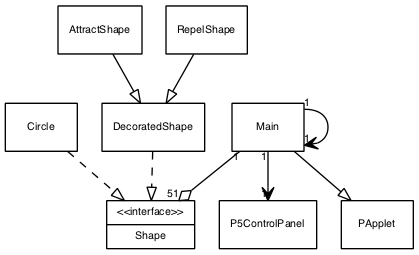
\includegraphics[width=.8\textwidth]{uml_simple.png}
	\caption{Diagrama de classes simplificado}
	\label{uml}
\end{figure}

\vspace{0.8 true cm}

\section{Funcionalidades}
\label{funcionalidades}

\vspace{0.4 true cm}
O programa inicia com 6 círculos em posições, direções e velocidades aleatórias, além de um ponto no centro da tela representando o centro de 
massa de atração\/repulsão. Outros comportamentos podem ser adicionados a partir das seguintes teclas ou botões:
\vspace{0.4 true cm}
\begin{description}

\item[Botão Vectors] \hfill \\
Mostra/esconde o vetor de direção do círculo.
\vspace{0.4 true cm}

\item[Botão Connect] \hfill \\
Mostra/esconde as linhas que ligam os centros de todos os círculos.
\vspace{0.4 true cm}

\item[Botão Attract] \hfill \\
Atrai todos os círculos para o centro de massa.
\vspace{0.4 true cm}

\item[Botão Repel] \hfill \\
Aumenta a repulsão entre os círculos.
\vspace{0.4 true cm}

\item[Botão Reset] \hfill \\
Desfaz todos os comportamentos adicionados, retornando a execução ao estado inicial.
\vspace{0.4 true cm}

\item[Botão Trail] \hfill \\
Diminui a frequência de atualização do background da tela, ou seja, diminui a taxa na qual o fundo da tela é redesenhado, 
mantendo desenhos antigos na tela.
\vspace{0.4 true cm}

\item[Botão Size] \hfill \\
Aumenta/reduz o tamanho dos círculos.
\vspace{0.4 true cm}

\item[Botão RepelIntensity] \hfill \\
Aumenta/reduz a distância de repulsão entre os círculos.
\vspace{0.4 true cm}

\item[Barras horizontais] \hfill \\
Alteram a cor das linhas criadas pelo botão Connect, sendo as 3 primeiras barras referentes às cores RGB e a última referente à opacidade.
\vspace{0.4 true cm}

\item[Botão Add] \hfill \\
Adiciona um novo círculo, sendo o máximo possível igual a 30.
\vspace{0.4 true cm}

\item[Botão Remove] \hfill \\
Remove o último círculo adicionado contanto que o número de círculos na tela seja maior que 5.
\vspace{0.4 true cm}

\item[Tecla Espaço] \hfill \\
Adiciona um círculo atrator, sendo o máximo possível igual a 10. Não é afetado pelas demais funcionalidades, exceto pelo \textit{Trail}.
\vspace{0.4 true cm}

\item[Tecla Enter] \hfill \\
Adiciona um círculo repelidor, sendo o máximo possível igual a 10. Também é afetado somente pelo \textit{Trail}.
\vspace{0.4 true cm}

\item[Tecla Tab] \hfill \\
Mostra/esconde o menu de opções.
\vspace{0.4 true cm}

\item[Tecla Shift + P] \hfill \\
Tira um screenshot da tela e salva na pasta \textit{prints}

\end{description}

\section{Testes}
\label{testes}

O desenvolvimento deste aplicativo passou por diversas fases até chegar ao estado de arte em que se encontra. Por se tratar também de um conceito
que pode ser considerado bastante abstrato por alguns, não havia, inicialmente, uma ideia fixa de como seria o estado final do programa. Assim,
seguem algumas imagens das primeiras versões e ideias que tivemos, que podem ser consideradas também como testes para descobrirmos os potenciais
que poderiamos atingir, além de servir como motivação para a evolução incremental da ideia.

\begin{figure}[H]
  \centering
  \begin{minipage}{.5\textwidth}
    \centering
    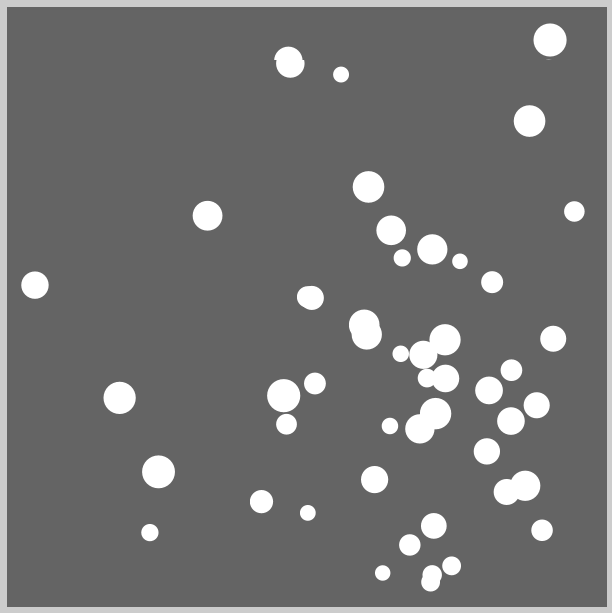
\includegraphics[scale=0.35]{firstver}
    \caption{v0.1}
  \end{minipage}%
  \begin{minipage}{.5\textwidth}
    \centering
    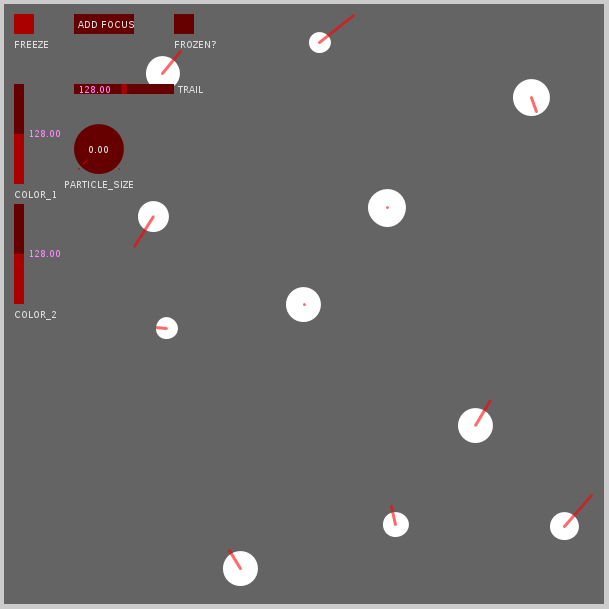
\includegraphics[scale=0.35]{secondver}
    \caption{v0.5}
    \end{minipage}%
\end{figure}
    

\begin{figure}[H]
  \centering
  \begin{minipage}{.5\textwidth}
    \centering
    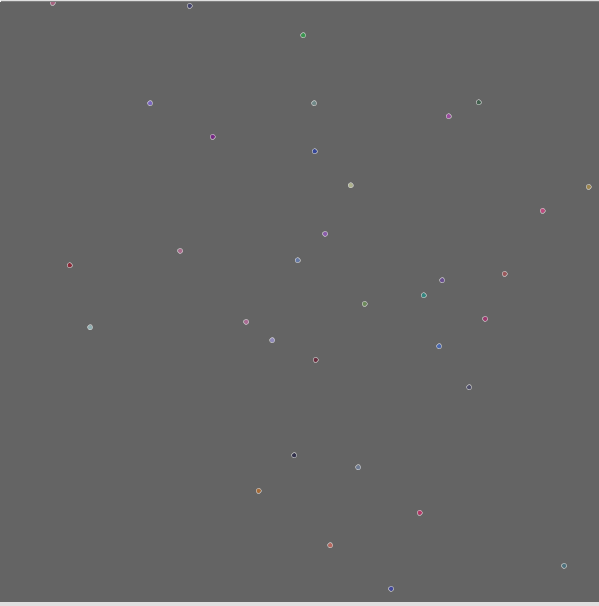
\includegraphics[scale=0.35]{experiment}
    \caption{v0.8}
  \end{minipage}%
  \begin{minipage}{.5\textwidth}
    \centering
    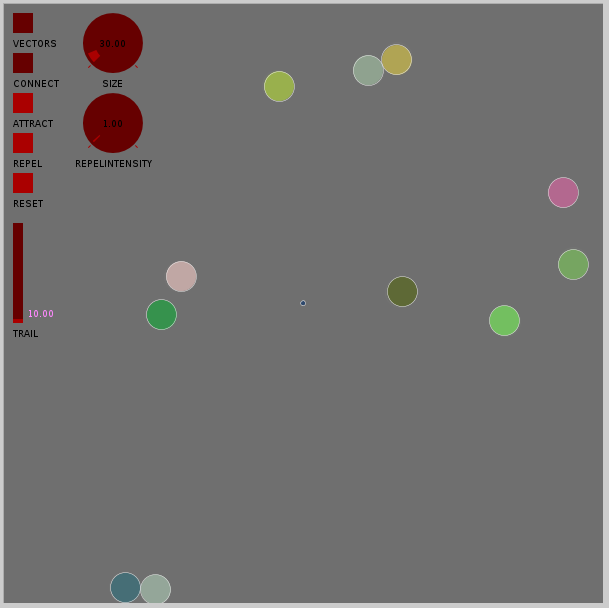
\includegraphics[scale=0.35]{thirdver}
    \caption{v1.0}
    \end{minipage}%
\end{figure}

\section{Conclusão}
\label{conclusao}
A partir deste trabalho foi possível aprimorar nossos conhecimentos em programação modular pela aplicação conceitos de padrões de projeto, 
interface gráfica, herança e encapsulamento de dados. Além do mais, o projeto também proporcionou uma experiência de desenvolvimento em equipe
e da modelagem em conjunto de um problema, aproximando-nos à realidade de desenvolvimento do mercado.

Apesar das dificuldades de implementação do padrão de projeto Decoratir, os resultados mostraram-se satisfatórios e até mesmo melhores do que
o esperado. Gerar padrões de imagens mostrou-se bastante divertido e foram gastos horas apenas experimentando as diversas combinações de funcionalidades

\bibliographystyle{sbc}
\bibliography{tp1}

\begin{figure}[h!]
	\centering
	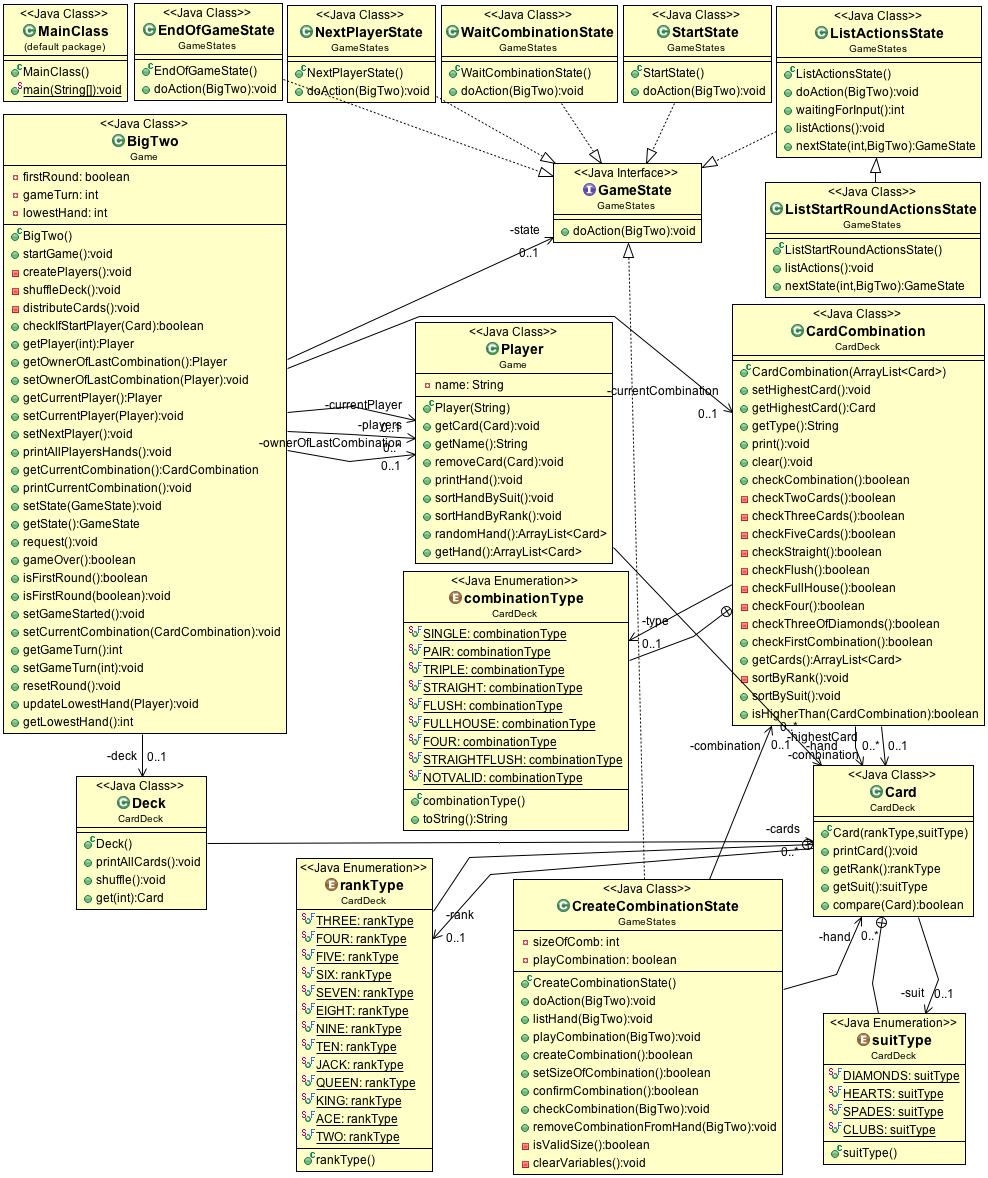
\includegraphics[width=.8\textwidth]{umlfull.png}
	\caption{Diagrama de classes completo}
	\label{umlfull}
\end{figure}

\end{document}
